\documentclass[12pt]{scrartcl}
\usepackage[utf8]{inputenc}
\usepackage[ngerman]{babel}
\usepackage[T1]{fontenc}
\usepackage{bm}
\usepackage{amsmath}
\usepackage{amssymb}
\usepackage{graphicx}
\usepackage{stmaryrd}
\usepackage{hyperref}
\usepackage[font=small]{caption}
%\captionsetup{format=plain}
\usepackage{enumitem}
\parindent0pt
\sloppy
\usepackage{float}
\newcommand\tab[1][1cm]{\hspace*{#1}}

\title{Julia Fraktale}
\date{25.Juli.2021}
\author{-}

\begin{document}
\begin{titlepage}
\centering
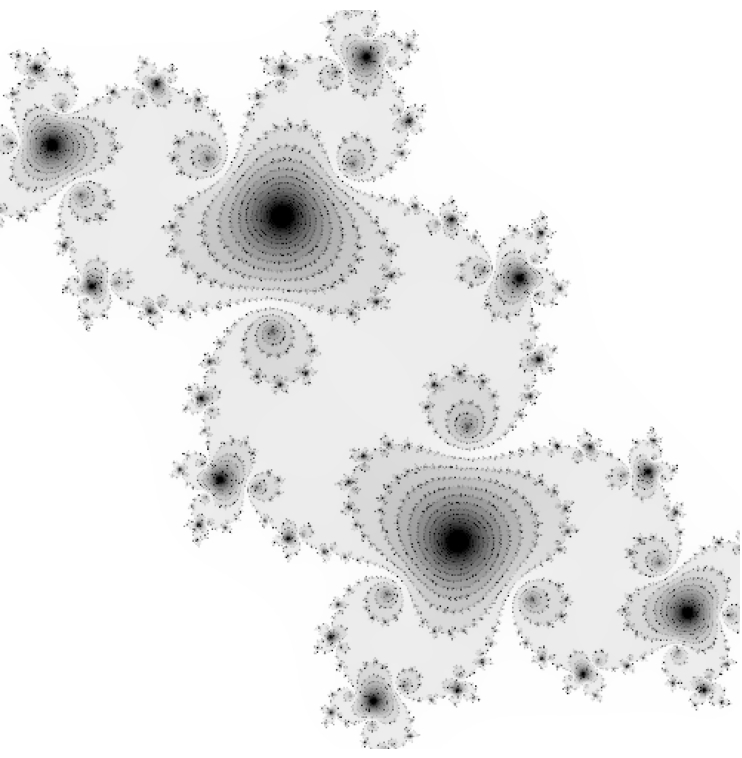
\includegraphics[scale=0.3]{Titel.jpg}\par
\vspace{1.5cm}
{\scshape\LARGE Universität Stuttgart \par}
\vspace{1.5cm}
{\scshape\Large Mathematische Programmierung Projektarbeit 1\par}
\vspace{1.5cm}
{\small Aufgabe 1\par}
{\huge\bfseries Julia Fraktale\par}
\vspace{1.5cm}
{\Large\itshape -\par}
\vfill
{\large 25.Juli.2021\par}
\end{titlepage}


\tableofcontents
\newpage

\section{Vorwort}
Es sei erwähnt, dass dieses Dokument mit \LaTeX verfasst.\\
Variablen wurden in \texttt{Schreibmaschinenschrift} geschrieben und explizite Code-Zeilen zusätzlich zentriert. Die Namen von Funktionen wurde \textit{kursiv} verfasst.\\
Alle verwendeten Bilder wurden mit \glqq Julia Fraktale.py\grqq ~erzeugt und die exakten Code-Zeilen befinden sich in Kapitel \ref{Anhang}.

\section{Externe Module}
Folgende Module wurden verwendet:
\begin{center}
\begin{tabular}{|p{4cm}|p{2.4cm}|p{7.6cm}|}
\hline
\textbf{Name} & \textbf{Abkürzung} & \textbf{Zweck} \\
\hline \hline
matplotlib.pyplot & plt & Darstellung einer Matrix als Bild \\
\hline
matplotlib.animation & animation & Animation der Generierung \\
\hline
numpy & np & Für große mathematische Operationen \\
\hline
math & - & Für Beispiele mit $\pi$ und $e$\\
\hline
\end{tabular}
\end{center}

Da es sich hierbei ausschließlich um Standartmodule handelt, wurden diese dem Projekt nicht beigelegt.

\section{Parameter}
\subsection{brightness}
Die Funktion \textit{brightness} verwendet folgende Parameter:

\begin{center}
\begin{tabular}{|p{2cm}|p{2cm}|p{2.8cm}|p{7cm}|}
\hline
\textbf{Name} & \textbf{Datentyp} & \textbf{Standartwert} & \textbf{Zweck} \\
\hline \hline
\texttt{f} & np.poly1d & - & Die Funktion von der die Julia-Menge gebildet werden soll \\
\hline
\texttt{M} & int & 500 & Ergibt quadriert die Anzahl der betrachteten Punkte \\
\hline
\texttt{N} & int & 1000 & Maximale Anzahl der betrachteten Potenzen von f \\
\hline
\texttt{R} & float & 2 & Schranke, ab der aufgehört wird weitere Potenzen von f zu betrachten \\
\hline
\texttt{I} & list & [-1, 1] & Unter und obere Grenze des betrachteten Intervalls \\
\hline
\texttt{name} & str & out & Name des Bildes, was am Schluss gespeichert wird \\
\hline
\texttt{animation} & bool & False & Ob das Fraktal animiert werden soll \\
\hline
\texttt{save} & bool & False & Ob das Fraktal gespeichert werden soll \\
\hline
\end{tabular}
\end{center}

\subsection{animate}
Die Funktion \textit{animate} verwendet folgende Parameter:

\begin{center}
\begin{tabular}{|p{2cm}|p{2cm}|p{2.8cm}|p{7cm}|}
\hline
\textbf{Name} & \textbf{Datentyp} & \textbf{Standartwert} & \textbf{Zweck} \\
\hline \hline
frame & int & - & Das Frame zu welchem das entsprechende Bild ausgegeben werden soll.\\
\hline
\end{tabular}
\end{center}


\section{Features}
Wie die oben beschriebenen Variablen schon angedeutet haben, besitzt die hier verwendete Visualisierungsmethode zusätzlich zu den von der Aufgabenstellung geforderten Eigenschaften noch folgende Features:
\begin{itemize}
\item[-] Eine Fortschrittsanzeige\\
Der prozentuale Fortschritt wird, wie in Abb. \ref{Fortschritt} gezeigt, in der Konsole ausgegeben.
\item[-] Personalisierte Namen\\
Über einen String kann man den Namen des ausgegebenen Bildes frei wählen.
\item[-] Speichern als .png\\
Über den Wahrheitswert der Variablen \texttt{save} lässt sich das Bild mit dem gewählten Namen direkt abspeichern.
\end{itemize}

\begin{figure}[H]
\centering
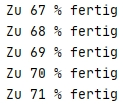
\includegraphics[scale=1]{Fortschritt.jpg}
\caption{}
\label{Fortschritt}
\end{figure}

\section{Dokumentation}
\subsection{Lokale Variablen}
In diesem Abschnitt wird die Bedeutung der Verwendeten Variablen erklärt.\\

Die Variable \texttt{h} ist ein 2D-Array der Dimension \texttt{M}x\texttt{M}. In diesem Array werden die Helligkeitswerte der jeweiligen komplexen Zahl gespeichert und dementsprechend die Helligkeit dieses Pixels.\\

\texttt{H} ist quasi der große Bruder von \texttt{h}. Dies wird nur dann erzeugt, wenn \texttt{animate} True ist. Es ist, wie \texttt{h}, von der Dimension \texttt{M}x\texttt{M}. besitzt aber zudem noch eine Tiefe von \texttt{N}/10, was später bei der Initialisierung in Kapitel \ref{Initialisierung} näher erläutert wird.\\

In \texttt{A} läuft der eigentliche Rechen- und Iterationsprozess (Kapitel \ref{Iteration}) ab, daher hat es ebenso die Dimension \texttt{M}x\texttt{M}. Hierbei ist aber wichtig, dass dieses Numpy-Array komplexe Zahlen enthält.\\

Die Variablen \texttt{X} und \texttt{Y} sind ähnlich aufgebaut. Beide sind Listen bestehend aus \texttt{M} Elementen, welche gleichmäßig verteile Zahlen zwischen Intervallanfangs- und Endpunkt enthalten.\\

\texttt{n} und \texttt{s} sind Laufvariablen, wobei erstere die momentane Iteration angibt und letztere die Schicht von \texttt{H}, was später noch erklärt wird (Kapitel \ref{Iteration}).\\

\texttt{T} ist eine Liste, welche speziell ausgewählte Koordinaten von Punkten aus A enthält.\\

\texttt{axis} ist offensichtlicherweise die Variable, welche die Grenzen der Ebene beschreibt und somit später die Achsenbeschriftung (Kapitel \ref{Vom_Array_zum_Bild}).\\

Dies waren alle Variablen aus \textit{brightness}.\\

Neben zuvor beschriebenen \texttt{I} und \texttt{axis} enthält \textit{animate} die Variable S, welche eine Teilmenge von \texttt{H} und damit ein \texttt{M}x\texttt{M} Array ist (Kapitel \ref{Vom_Array_zum_Bild}).

\subsection{Umsetzung}
Wie der Name \textit{brightness} andeutet, ist das Ziel dieser Funktion ein Array auszugeben, welches Helligkeitswerte enthält, mit welchen man ein Bild erzeugen kann. Dies wurde dann in soweit erweitert, dass nun auch die Ausgabe des Bildes Teil dieser Funktion ist.\\\subsubsection{Initialisierung}\label{Initialisierung}


Für die Helligkeit gibt es 3 Fälle:
\begin{enumerate}[label=\arabic*.]
\item \label{1} Fall\\
Falls $|z| > \texttt{R}$ ist $h(z) = 1$
\item \label{2} Fall\\
Falls $|f^n(z)| > \texttt{R}$ aber für alle $k \leq n \leq \texttt{N}$ $|f^k(z)| \leq \texttt{R}$ ist $h(z) = 1 - \dfrac{n}{\texttt{N}}$
\item \label{3} Fall\\
Falls $|f^k(z)| \leq \texttt{R}$ für alle $k \leq \texttt{N}$ ist $h(z) = 0$
\end{enumerate}

Der \ref{3} Fall ist direkt durch die anfängliche Erzeugung von \texttt{h} geklärt, denn es gilt:\\

\tab \texttt{h = np.zeros(shape = (M, M))}~~~.\\

Also h wird als Array voller Nullen erzeugt. Die Einträge werden nur verändert, falls einer der anderen Fälle eintritt.\\

Ähnlich wie \texttt{h} wird, wenn \texttt{animation} True ist,\\

\tab \texttt{H = np.zeros(shape = (int(N / 10) + 1, M, M))}\\

erzeugt. Es sei an dieser Stelle darauf hingewiesen, dass der Animationsprozess somit nicht für \texttt{N} mod 10 $\neq$ 0 funktioniert.\\

\texttt{A} wird genau wie \texttt{h} erzeugt.\\

Die Listen \texttt{X} und \texttt{Y}, welche den Real- und Imaginärteil von $z$ darstellen werden durch \texttt{np.linspace} erzeugt, was dafür sorgt, dass man die geforderten gleichmäßig verteilten Punkte erhält.\\

Durch die \texttt{for}-Schleife\\

\tab \texttt{for y in range(len(Y)):\\
        \tab \tab for x in range(len(X)):\\
            \tab \tab \tab A[y, x] = complex(X[x], Y[y])}\\

werden alle \texttt{x} $\in$ \texttt{X} und \texttt{y} $\in$ \texttt{Y} durchlaufen und \texttt{A} an der entsprechenden Stelle mit der komplexen Zahl z = \texttt{x} + \texttt{y} $\cdot~i$ $\in \mathbb{C}$ ersetzt.\\

An dieser Stelle wird auch der \ref{1} Fall geprüft:\\

\tab \texttt{if np.abs(A[y, x]) > R:} \\
\tab \tab \texttt{h[y, x] = 1}~~~.\\

\subsubsection{Iteration}\label{Iteration}
Der nächste Teil ist quasi das Herzstück der gesamten Funktion. Hier läuft der Iterationsprozess und somit auch der noch fehlende \ref{2} Fall ab.\\

Die \texttt{while}-Schleife läuft solange \texttt{n} $\leq$ \texttt{N} ist.\\

\tab \texttt{A = np.where((np.abs(A) <= R) \& (np.abs(A) != R**2 + 10), f(A), A)}\\

Dies durchsucht das Array nach Einträgen $a$, welche $|a| \leq \texttt{R}$ und $|a| \neq \texttt{R}^2 + 10$ erfüllen. An einer solchen Stelle wird der Eintrag von \texttt{A} durch \texttt{f(A)} ersetzt. Ansonsten bleibt er unverändert.\\
$\texttt{R}^2 + 10$ wurde so gewählt, damit ein Wert konstruiert wird, welcher nie \glqq aus versehen\grqq ~angenommen wird.\\

Die nächste Zeile beschäftigt sich mit dem \ref{2} Fall:\\

\tab \texttt{T = list(zip(*np.where((np.abs(A) > R) \& (A != R**2 + 10))))}\\

Diese sehr komplizierte Schreibweise erzeugt eine Liste \texttt{T}, welche die Koordinaten der Einträge $a$ aus \texttt{A} enthält, welche $|a| > \texttt{R}$ und $|a| \neq \texttt{R}^2 + 10$ erfüllen, was eben genau der \ref{2} Fall ist.\\

Die Elemente dieser Liste werden mit einer \texttt{for}-Schleife durchlaufen und manipulieren \texttt{h} und \texttt{A} an den entsprechenden Stellen so, dass \texttt{h} an dieser Stelle gleich $1 - \texttt{n}/\texttt{N}$ und \texttt{A} auf den Sperrwert $\texttt{R}^2 + 10$ gesetzt wird.\\

Der nächste Teil beschäftigt sich mit dem Fall das \texttt{N} mod 10 = 0 ist. Falls \texttt{animation} == True wird\\

\tab \texttt{H[s] = h}~~~,\\

also wird \texttt{H} alle 10 Iterationen in der Schicht \texttt{s} auf den momentanen Stand von \texttt{h} gesetzt. Dies sind dann später die \texttt{frames} der Animation (Kapitel \ref{Vom_Array_zum_Bild}). Anschließend wird \texttt{s} um 1 erhöht.\\

Des Weiteren wird im Fall \texttt{N} mod 10 = 0 der prozentuale Fortschritt über den \texttt{print}-Befehl ausgegeben.\\

Damit die \texttt{while}-Schleife irgenwann terminiert wird schlussendlich \texttt{n} um eins erhöht.

\subsubsection{Vom Array zum Bild}\label{Vom_Array_zum_Bild}
Der nun folgenden Teil beschäftigt sich mit der Darstellung eines Array durch \texttt{matplotlib}.\\

\tab \texttt{plt.imshow(h, cmap = "gray", vmin = 0, vmax = 1, extent = axis)}\\

spielt hierbei die zentrale Rolle.\\
Als \glqq Farbe\grqq ~wird hier \texttt{gray}, also Graustufen verwendet, sodass für den Arrayeintrag \texttt{0} Schwarz und für \texttt{1} Weiß erzeugt wird. Schlussendlich wird mit \texttt{extent} die Achsenbeschriftung erzeugt.\\

Nun wird noch im Falle, dass \texttt{save} gewünscht ist, der \texttt{plot} als \texttt{name}.png gespeichert und mit \texttt{plt.show()} angezeigt.\\

Die Ausgabe von \textit{brightness} hängt davon ab, ob \texttt{animation} gefordert ist. In diesem Fall wird \texttt{H} zurückgegeben und ansonsten \texttt{h}.

\subsubsection{Animation}
Die Funktion \textit{animate} erzeugt basierend auf der Nummer des frames und somit der framten Schicht von \texttt{H}, welche mit \texttt{S} bezeichnet ist, über \texttt{im.show(\dots)} wie oben das Bild \texttt{im}, was schlussendlich auch die Ausgabe von \textit{animate} ist.

\subsubsection{Polynome}
Das Ende des Codes bilden einige Aufrufe von \textit{brightness} zu verschiedenen Polynomen \texttt{f}, \texttt{R} und \texttt{N}, welche in Kapitel \ref{Bilder_und_Beispiele} genauer erläutert werden.\\

\tab \texttt{animation.FuncAnimation(fig, animate, frames = 100, interval = 200, \\ \tab \tab blit = True)}\\

erzeugt die in (d) geforderte Animation mit \texttt{matplotlib.animation}. Mit insgesamt 100 Bildern und 0,2 Sekunden Pause zwischen den Bilder, also 5 fps.

\section{Benutzungshinweise}
Dank der Ausgabe des Fortschritts lässt sich leicht nachvollziehen, ob das Programm läuft. Die Berechnung dauert auf meinem PC\footnote[1]{Intel i7-6700K, 32GB RAM, NVIDIA GTX 980 Ti} für alle Polynome jeweils unter 20 Sekunden.\\

Eigene Julia-Fraktale lassen sich über den Aufruf der \textit{brightness}-Funktion relativ einfach erzeugen.
Es wird nur ein Polynom benötigt. Wenn man ein \glqq einfaches\grqq ~Julia-Fraktal erstellen möchte, braucht man einen Ausdruck der Form $\texttt{f}(z) = z^2 + c$ mit $c \in \mathbb{C} \setminus \mathbb{R}$.\footnote[2]{mit reellen c ist es langweilig}\\
Demnach ist bei \texttt{np.poly1d([1,0, complex(a, b)])} noch die (komplexe) Konstante \texttt{a} + \texttt{b} $\cdot ~i$ zu wählen.\\

Man kann nach belieben mit den Variablen \texttt{M}, \texttt{N}, \texttt{R} und \texttt{I} spielen. Es sei aber zu beachten, dass der Rechenaufwand für \texttt{M} quadratisch und für \texttt{N} linear ansteigt.\\

Wenn man sein wunderschönes Fraktal gerne als .png haben wöllte, muss die Funktion mit \texttt{save = True} übergeben werden.\\

Wer eine Animation seines Polynoms sehen will, muss das Polynom in\\

\tab \texttt{H = brightness(f = np.poly1d([1, 0, complex(-0.1, 0.651)]), name = \\ \tab \tab \dq Atoll", animation = True, save = True)}\\

ändern.\\
Falls man ein anderes \texttt{N} möchte, funktioniert die Animation nur, wenn man in \texttt{animation.FuncAnimation} die \texttt{frames} auf \texttt{N}/10 setzt. Veränderte Intervallgrenzen müssen \textit{brightness} übergeben werden und in \textit{animate} entsprechend verändert werden.

\section{Bilder und Beispiele}\label{Bilder_und_Beispiele}
Die Fraktale erhielten Name je nachdem wonach sie aussahen; diese werden hier als Überschriften verwendet und die exakten Einstellungen, die zu den Bilder führten werden im Anhang (Kapitel \ref{Anhang}) beschrieben.

\subsection{Atoll}

\begin{figure}[H]
\centering
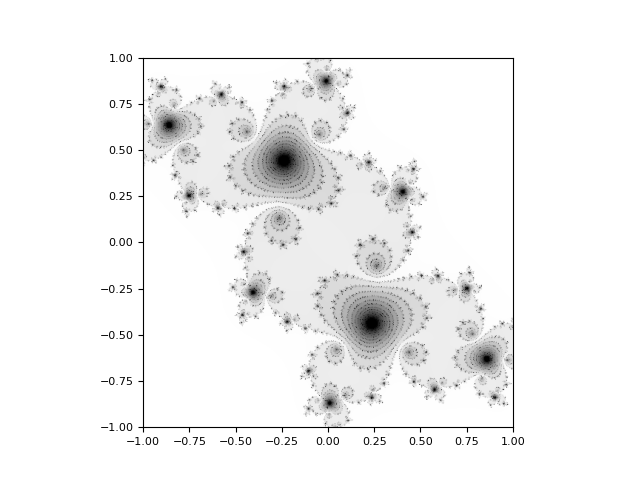
\includegraphics[scale=0.5]{Atoll0.png}
\caption{}
\label{Atoll0}
\end{figure}


Dies ist das Fraktal zu (c) also $\texttt{f}(z) = z^2 - 0.1 + 0.651 \cdot i$.

\subsection{Elefant}

\begin{figure}[H]
\centering
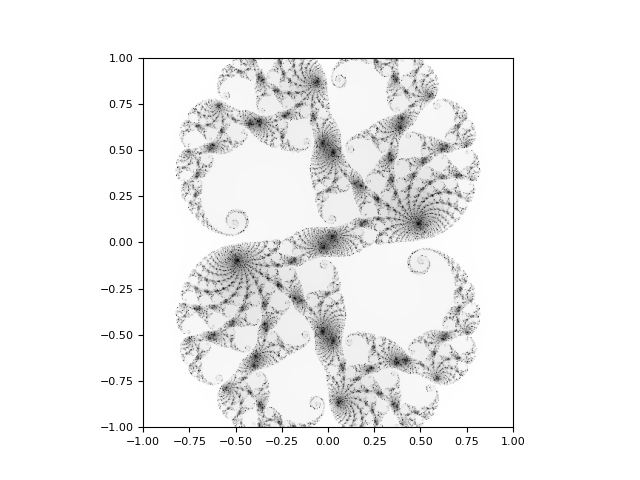
\includegraphics[scale=0.5]{Elefant0.png}
\caption{}
\label{Elefant0}
\end{figure}

Dies ist ein Fraktal zu $\texttt{f}(z) = z^2 + 0.26 + 0.0016 \cdot i$.

\subsection{Illusion}

\begin{figure}[H]
\centering
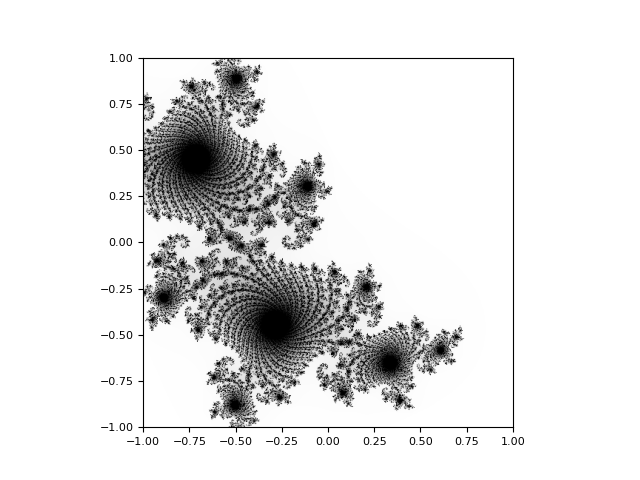
\includegraphics[scale=0.5]{Illusion0.png}
\caption{}
\label{Illusion0}
\end{figure}

Dies ist ein Fraktal zu $\texttt{f}(z) = z^2 + z - 0.306 + 0.648 \cdot i$ mit \texttt{N} = 500.\footnote[3]{Wenn man auf die großen schwarzen Punkte schaut, scheinen diese größer zu werden. Ich kann Ihnen aber versichern, dass dies nur ein Bild ist und es demnach eine optische Illusion sein muss.}

\subsection{Fancy}
Manche Leute behaupt $e^{i \cdot \pi} - 1 = 0$ sei die schönste Gleichung der Mathematik, da sie die wichtigen Konstanten $e$, $\pi$ und $i$ mit den neutralen Elementen der Multiplikation und Addition verbinden.\\
Wem das gefällt, wird auch folgendes Fraktal gefallen:\\

\begin{figure}[H]
\centering
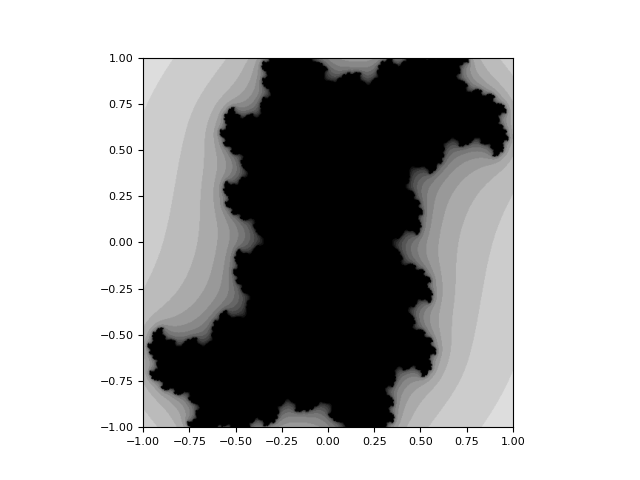
\includegraphics[scale=0.5]{Fancy0.png}
\caption{}
\label{Fancy0}
\end{figure}

Dies ist ein Fraktal zu $\texttt{f}(z) = z^2 + 1/\pi - 1/e \cdot i$ mit \texttt{R} = 15 und \texttt{N = 15}.\\
Es verbindet also genauso diese schönen Zahlen.\footnote[4]{Die $0$ kann man einfach gedanklich dazu addieren.}

\section{Variation der Variablen}
Abschließend stellt sich noch die Frage: Wie beeinflussen die Variablen das Fraktal?\footnote[5]{Der Titel wurde in Anlehnung an die \glqq Variation der Konstanten\grqq ~gewählt.}

\subsection{\texttt{f}}
Das betrachtete Polynom \texttt{f} beeinflusst grundlegend die Struktur, wie man an den oberen Beispielen leicht erkennen kann.\\
Eine Animation von verschiedenen Polynomen $f_c(z) = z^2 + c$ lässt sich in diesem Video\footnote[6]{https://youtu.be/fAsaSkmbF5s?t=788} anschauen.

\subsection{\texttt{M}}
Die Variation von \texttt{M} verändert die Auflösung des Bildes:\\

\begin{figure}[H]
\centering
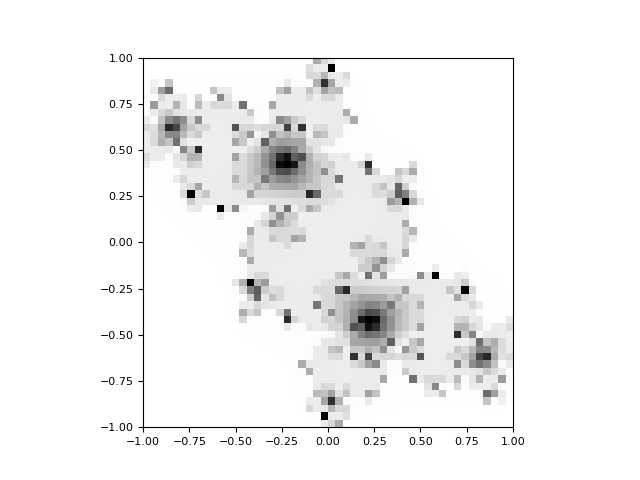
\includegraphics[scale=0.5]{Atoll1.png}
\caption{}
\label{Atoll1}
\end{figure}

Dies ist das Fraktal zu $\texttt{f}(z) = z^2 - 0.1 + 0.651 \cdot i$ und \texttt{M} = 50.\\
Offensichtlich ist es viel gröber gepixelt als das Bild von oben.

\subsection{\texttt{N}}
Die Variation von \texttt{N} verändert die Helligkeit:\\

\begin{figure}[H]
\centering
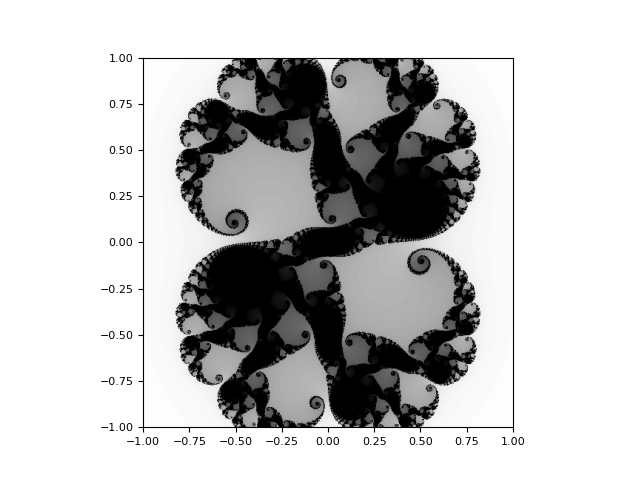
\includegraphics[scale=0.5]{Elefant1.png}
\caption{}
\label{Elefant1}
\end{figure}

Dies ist ein Fraktal zu $\texttt{f}(z) = z^2 + 0.26 + 0.0016 \cdot i$ und \texttt{N} = 100.\\

\begin{figure}[H]
\centering
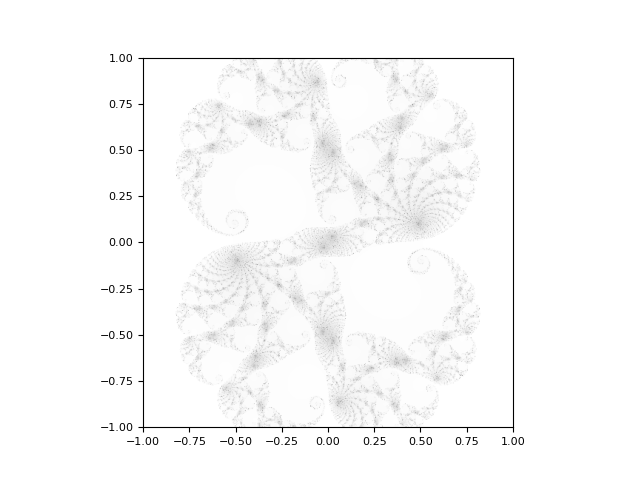
\includegraphics[scale=0.5]{Elefant2.png}
\caption{}
\label{Elefant2}
\end{figure}

Dies ist ein Fraktal zu $\texttt{f}(z) = z^2 + 0.26 + 0.0016 \cdot i$ und \texttt{N} = 4000.\\
Also größere \texttt{N} machen das Bild heller und kleinere dunkler.

\subsection{\texttt{R}}
Die Variation von \texttt{R} verändert die Helligkeit minimal.\\

\begin{figure}[H]
\centering
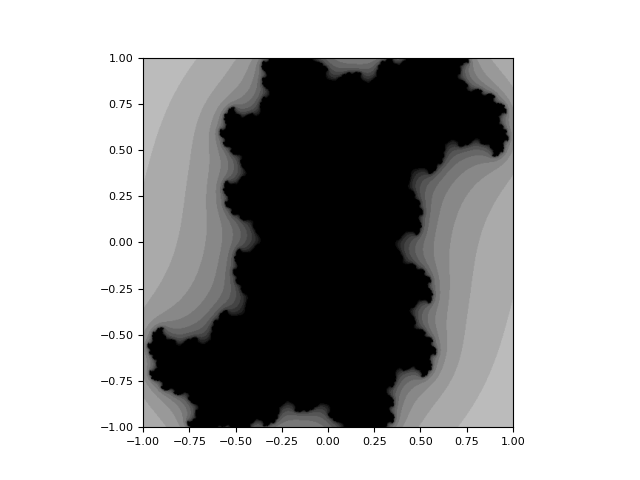
\includegraphics[scale=0.5]{Fancy1.png}
\caption{}
\label{Fancy1}
\end{figure}

Dies ist ein Fraktal zu $\texttt{f}(z) = z^2 + 1/\pi - 1/e \cdot i$ mit \texttt{R} = 5000 und \texttt{N = 15}.\\
Für kleine \texttt{N} wird das Bild für große \texttt{R} dunkler.

\subsection{\texttt{I}}
Die Variation von \texttt{I} verändert den betrachteten Bereich des Bildes.\\

\begin{figure}[H]
\centering
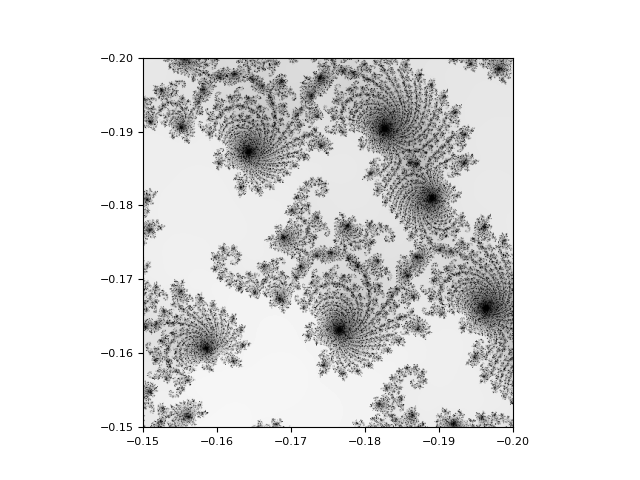
\includegraphics[scale=0.5]{Illusion1.png}
\caption{}
\label{Illusion1}
\end{figure}

Dies ist ein Fraktal zu $\texttt{f}(z) = z^2 + z - 0.306 + 0.648 \cdot i$ mit \texttt{I} = $[-0.15 , -0.2]$.

\newpage

\section{Anhang}\label{Anhang}
\begin{itemize}
\item[-] Abbildung \ref{Atoll0}\\
\texttt{brightness(f = np.poly1d([1, 0, complex(-0.1, 0.651)]), name = \dq Atoll", save = True)}
\item[-] Abbildung \ref{Elefant0}\\
\texttt{brightness(f = np.poly1d([1,0, complex(0.26, 0.0016)]), name = \dq Elefant", save = True)}
\item[-] Abbildung \ref{Illusion0}\\
\texttt{brightness(f = np.poly1d([1, 1, complex(-0.306, 0.648)]), N = 500, name = \dq Illusion", save = True)}
\item[-] Abbildung \ref{Fancy0}\\
\texttt{brightness(f = np.poly1d([1,0, complex(1/math.pi, -1/math.e)]), R = 15, N = 15, name = "Fancy", save = True)}
\item[-] Abbildung \ref{Atoll1}\\
\texttt{brightness(f = np.poly1d([1, 0, complex(-0.1, 0.651)]), M = 50, name = \dq Atoll", save = True)}
\item[-] Abbildung \ref{Elefant1}\\
\texttt{brightness(f = np.poly1d([1,0, complex(0.26, 0.0016)]), N = 100, name = \dq Elefant", save = True)}
\item[-] Abbildung \ref{Elefant2}\\
\texttt{brightness(f = np.poly1d([1,0, complex(0.26, 0.0016)]), N = 4000, name = \dq Elefant", save = True)}
\item[-] Abbildung \ref{Fancy1}\\
\texttt{brightness(f = np.poly1d([1,0, complex(1/math.pi, -1/math.e)]), R = 4000, N = 15, name = "Fancy", save = True)}
\item[-] Abbildung \ref{Illusion1}\\
\texttt{brightness(f = np.poly1d([1, 1, complex(-0.306, 0.648)]), I = [-0.15, -0.2], name = \dq Illusion", save = True)}
\end{itemize}

\end{document}